\chapter{Desenvolvimento}
\label{cap:desenvolvimento}







\section{Considerações Finais do Capítulo}
\label{sec:conclusao-desenvolvimento}

O capítulo abordou detalhadamente o processo de desenvolvimento do sistema inteligente proposto, organizando-se em três seções principais que tratam dos conjuntos de dados (Seção \ref{sec:aquisicao}), do modelo de aprendizagem profunda (Seção \ref{sec:modelo}) e do sistema de informação (Seção \ref{sec:si}). Essa estrutura reflete a integração dos componentes fundamentais que compõem a solução.

Inicialmente, a Seção \ref{sec:aquisicao} descreve os métodos de aquisição, organização e pré-processamento dos dados utilizados no treinamento do modelo. Os rótulos são provenientes do Galaxy Zoo, e as imagens são oriundas do DESI Legacy Survey. Um ponto de destaque é o ajuste do campo de visão angular, que assegura que as características morfológicas de interesse das galáxias sejam corretamente capturadas. Essa etapa é complementada pela limpeza e pela organização dos conjuntos de treinamento, validação, teste e inferência, garantindo representatividade e evitando viés nos resultados.

Em seguida, na Seção \ref{sec:modelo}, são apresentadas as etapas de desenvolvimento do modelo de aprendizagem profunda, incluindo o aumento de dados, a escolha das arquiteturas de rede neural e o ajuste de hiperparâmetros. Modelos como EfficientNet e DenseNet são explorados devido à sua eficiência em capturar padrões visuais complexos. Além disso, são discutidas métricas de avaliação, como a métrica mAP (mean Average Precision), que assegura a robustez e a precisão do modelo na tarefa de recuperação de imagens baseadas em similaridade visual.

A Seção \ref{sec:si} aborda a implementação dos componentes do backend, frontend e banco de dados. O sistema foi projetado para suportar a indexação eficiente de embeddings e realizar buscas rápidas por similaridade visual. Tecnologias como PostgreSQL e pipelines DevOps foram empregadas para garantir desempenho, escalabilidade e integração contínua. O frontend oferece uma interface intuitiva, permitindo aos usuários interagir facilmente com os dados e os resultados do sistema.

Por fim, a Fig. \ref{fig:diagrama-completo} sumariza todas as etapas desenvolvidas na solução. Os resultados obtidos serão abordados no próximo capítulo.

\begin{figure}[!ht]
  \centering
  \caption{Sumário do desenvolvimento do projeto}
  \label{fig:diagrama-completo}
  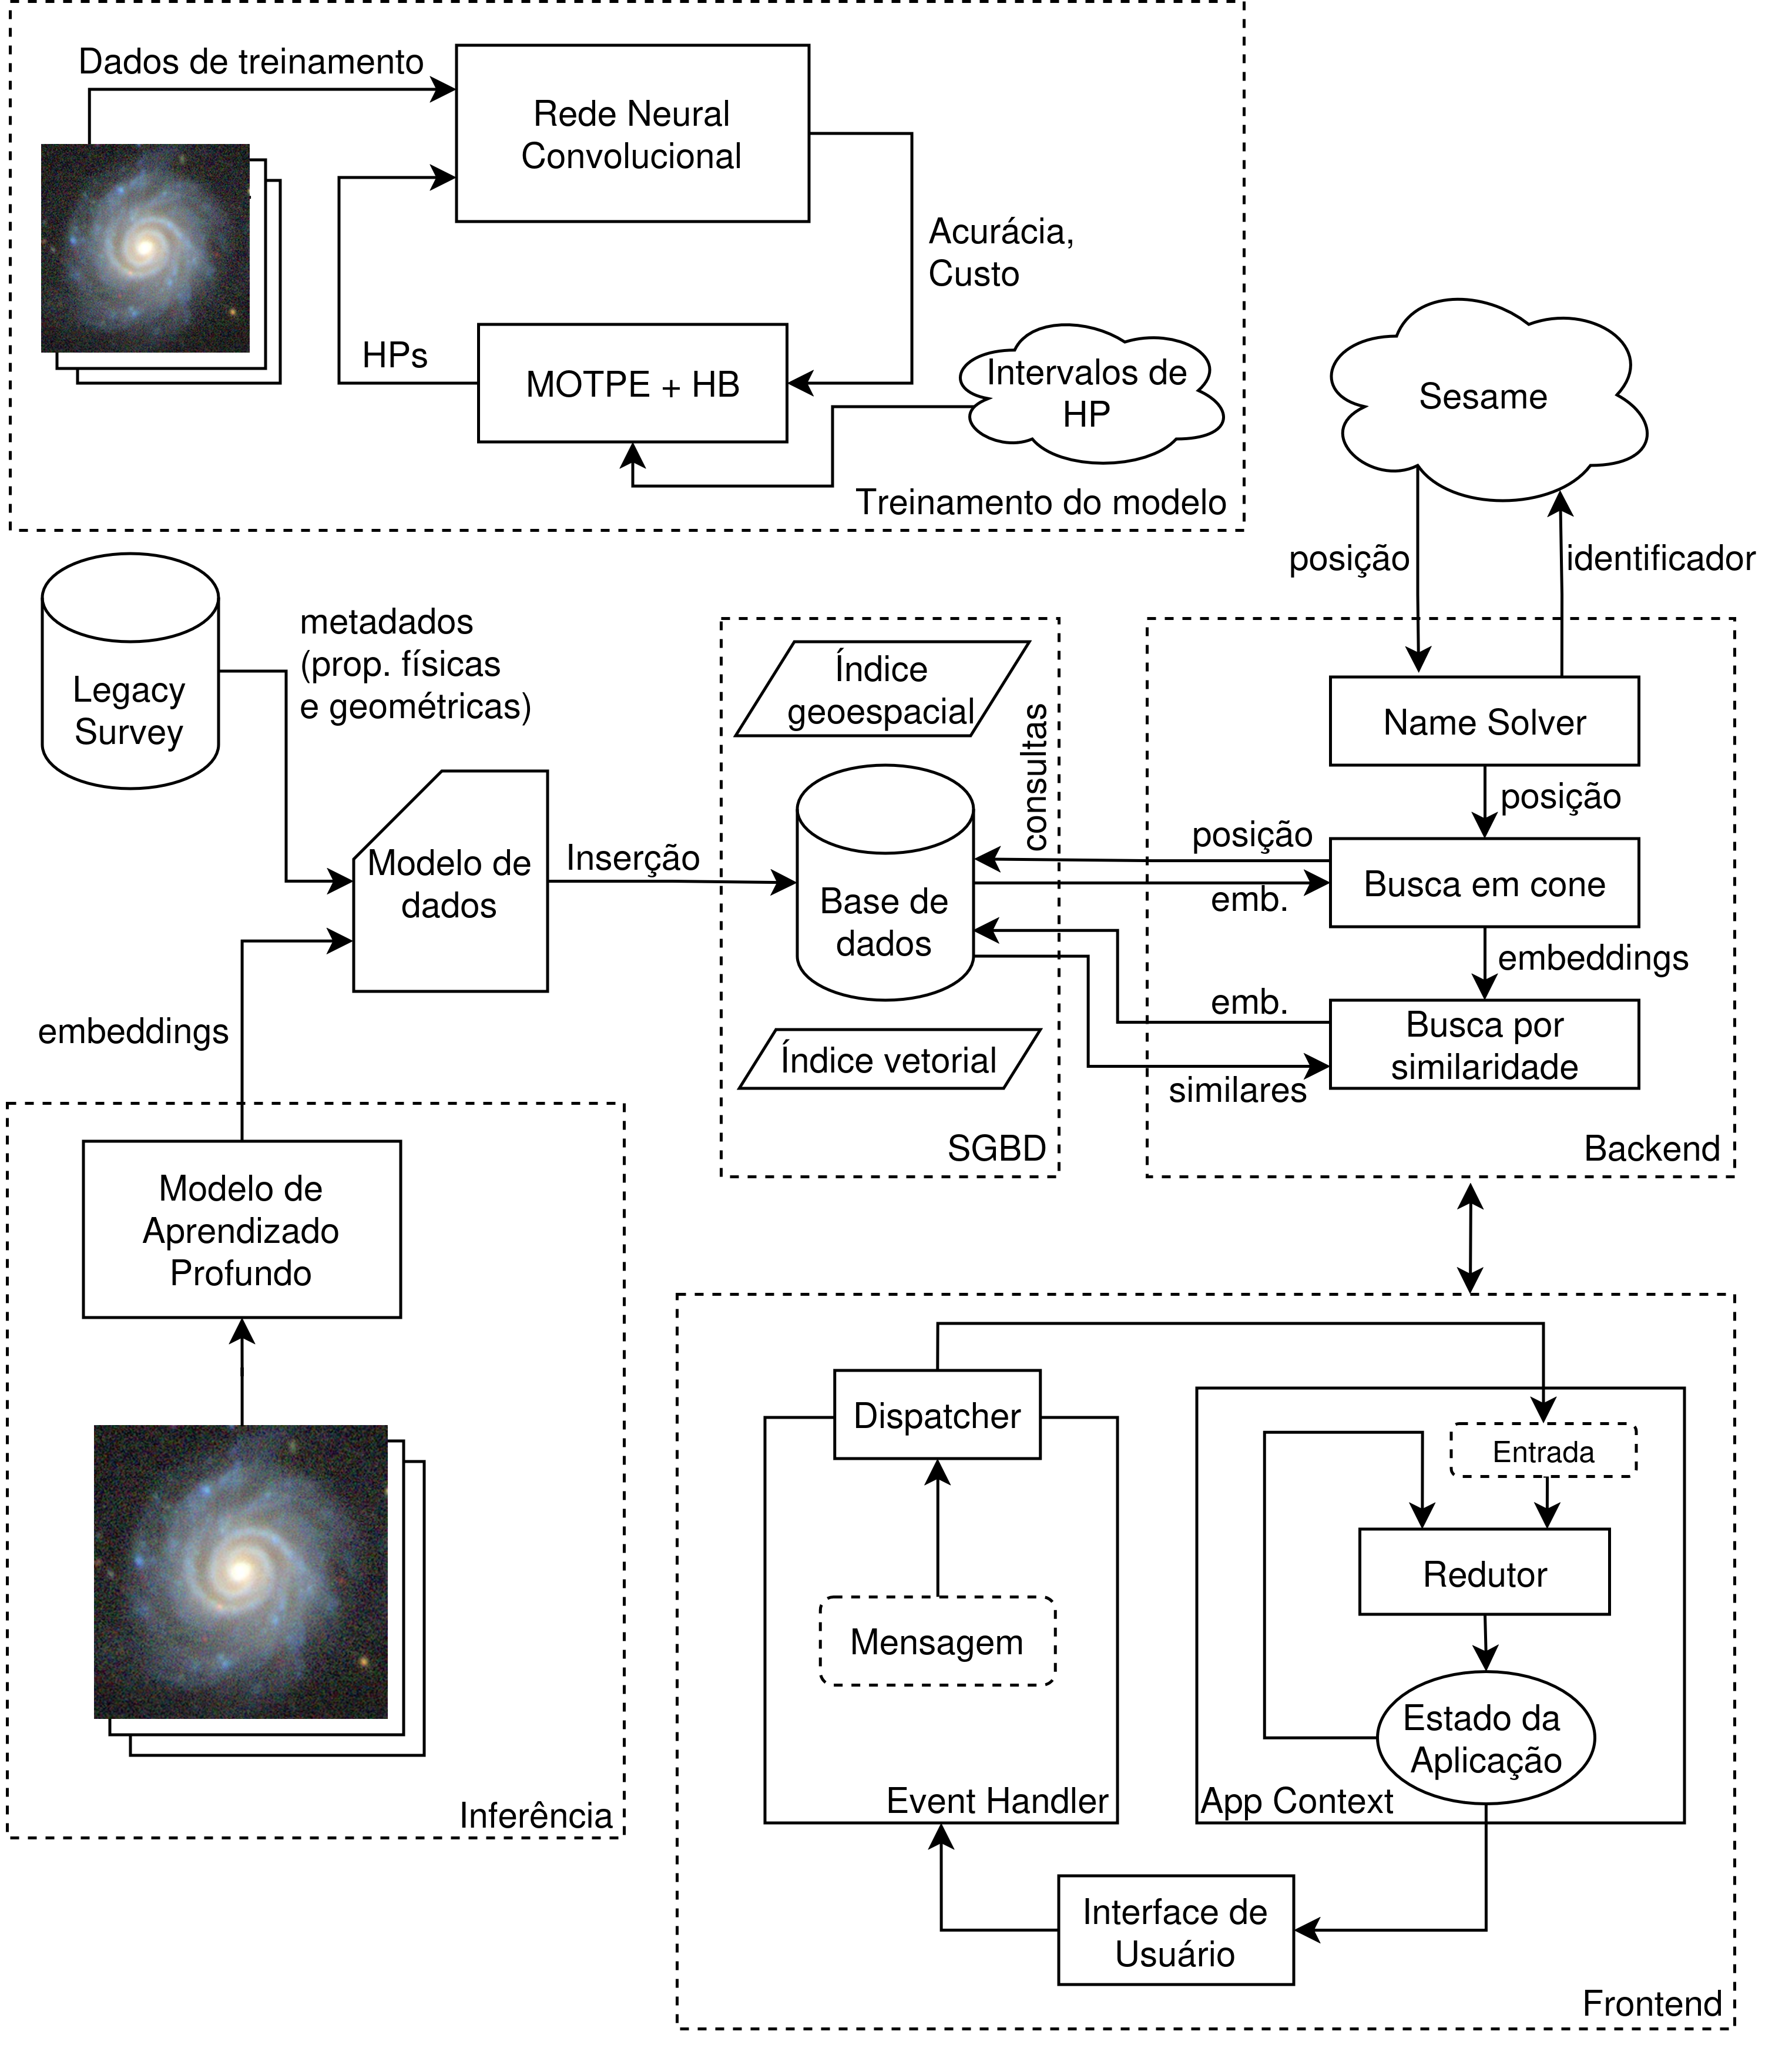
\includegraphics[width=\linewidth]{figures/full_diagram.png}
\end{figure}

\chaptersep


% \section{Conclusão do Capítulo}
